\documentclass[android.tex]{subfiles}
\usepackage{subfiles}
\documentclass[12pt,oneside]{memoir} 
\usepackage[latinica]{matfmaster} 

\begin{document}

Endi Rubin (\textit{Andy Rubin}) je 2003. godine sa trojicom kolega u Palo Altu osnovao kompaniju \textit{Android Inc. }sa namerom da kreiraju platformu za kameru sa podrškom za skladištenje u oblaku. Takva ideja nije naišla na podršku investitora i cilj kompanije se preusmerio na  pametne mobilne telefone, a vremenom i sve pametne uređaje. Zamisao je bila da sistem bude besplatan za korisnike, a da zarada zavisi od aplikacija i ostalih servisa. To je postalo moguće 2005. godine kada je kompanija \textit{Google} kupila kompaniju i ostavila priliku osnivačima na čelu sa Rubinom da nastave sa razvojem ovog operativnog sistema \cite{book:krajci}. 

Sam razvoj operativnog sistema i dalje traje, verzije su mnogobrojne i izlaze često, a svaka verzija donosi sa sobom znacajna poboljsanja
 \cite{sajt:androidDevelopers,book:mzivkovic}.  Svaka verzija je označena brojem, kao i nazivom slatkiša po ideji projektnog menadžera Rajana Gibsona. U tabeli \ref{tbl:andrVerzije} je prikazan pregled najznačajnijih verzija zajedno sa novitetima koje su donele. 

%%===================== TABELA =============================================================
\begin{table}
\centering
\caption{Verzije OS-a Android}
\label{tbl:andrVerzije}
\begin{tabular}{p{0.25\linewidth} | p{0.15\linewidth}p{0.6\linewidth}}
\toprule
Naziv verzije & Datum objavljivanja & Najznačajniji noviteti \\
\toprule
Android 1.0 & Septembar 2008. & Podrška za kameru, internet pregledač, preuzimanje i objavljivanje aplikacija na \textit{Android Market}-u, integrisani su \textit{Google} servisi: \textit{Gmail}, \textit{Google maps}, \textit{Google Calendar}, omogućene \textit{Wi-Fi} i \textit{bluetooth} bežične komunikacije\\\midrule
Android 1.5 - \textbf{\textit{Cupcake}} & April 2009. & Poboljšana \textit{Bluetooth} komunikacija, tastatura sa predikcijom teksta, snimanje i gledanje snimaka\\\midrule
Android 2.2 - \textbf{\textit{Froyo}} & Maj 2010. & Poboljšanje brzine, implementacija \textit{JIT}-a, instaliranje aplikacija van memorije telefona, povezivanje uređaja preko USB \\\midrule
Android 3.x - \textbf{\textit{Honeycomb}} & Februar 2011. & Višeprocesorska podrška, \textit{Google Talk} video čet, `\textit{Private browsing}`, uživo prenos preko HTTP-a, \textit{USB host API}, jednostavnije automatsko ažuriranje aplikacija preko \textit{Android Marketa}\\\midrule
Android 4.1-4.3 - \textbf{\textit{Jelly Bean}} & Jul 2012. & Glasovna pretraga, \textit{WiFi/WiFi-Direct} otkrivanje servisa, bezbedno USB debagovanje, 4K podrška, podrška za BLE (\textit{Bluetooth Low Energy}), \textit{WiFi scanning API}\\\midrule
Android 6.0 - \textbf{\textit{Marshmallow}} & Oktobar 2015. & Podrška za USB tip C, autentikacija pomoću otiska prsta, MIDI podrška\\\midrule
Android 8.0/8.1 - \textbf{\textit{Oreo}} & Avgust 2017. & Svetla i tamna tema, PIP (\textit{Picture-In-Picture}) sa opcijom promene veličine, API-ji za neuronske mreže i za deljenu memoriju\\\midrule
Android 9 - \textbf{\textit{Pie}} & Avgust 2018. & Prikaz celog teksta i slike u obaveštenjima o porukama, dugme za gašenje može i da snimi sliku ekrana\\\midrule
Android 10 - \textbf{\textit{Queen Cake}} & Septembar 2019 & Bolja podrška za privatnost, pristup sistemskim podešavanjima iz panela, biometrijska autentikacija unutar aplikacija\\\midrule
Android 11 - \textbf{\textit{Red Velvet Cake}} & Septembar 2020. & Snimak ekrana, balončići za poruke, podrška za 5G, bežično debagovanje, bolja podešavanja za dozvole\\\midrule
Android 12 - \textbf{\textit{Snow Cone}} & 2021. & \textit{Material You }jezik za dizajn, podrška za \textit{AVIF}, \textit{Android Private Compute Core}\\
\bottomrule
\end{tabular}
\end{table}
%===========================================================================================

Na pocetku razvoja, OS Android je svoju primenu našao u pametnim telefonima i tabletima. Tokom godina programeri su raširili upotrebu na media plejere (za Android TV), pametne satove i naočare, kućne uređaje, automobile, kamere, konzole za igru \cite{sajt:androidDevelopers}...   Prema statistici \cite{sajt:statistika}, Kineske kompanije drže više od 55\% Android tržišta. Od svih kompanija na tržištu najveći udeo imaju:\textit{ Samsung} (37.10\%), \textit{Xiaomi(}11.20\%) i \textit{Huawei}(11\%). Sa rastom raznovrsnosti aplikacija koje postoje za Android uređaje, kao i broja različitih uređaja koji se koriste rastao je i broj korisnika. Statistika vezana za trend rasta broja korisnika može se videti na slici \ref{fig:brKorisnika}.

%=================== SLIKA ======================================
\begin{figure}[!ht]
  \centering
  \label{fig:brKorisnika}
  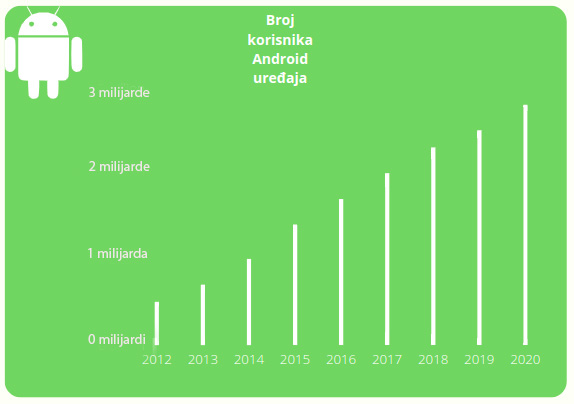
\includegraphics[width=0.9\textwidth]{brKorisnika.jpg}
  \caption{Broj korisnika tokom godina, izvor \cite{sajt:statistika}}
\end{figure}
%=====================================================================

\end{document}